\chapter{\IfLanguageName{dutch}{Stand van zaken}{State of the art}}
\label{ch:stand-van-zaken}

% Tip: Begin elk hoofdstuk met een paragraaf inleiding die beschrijft hoe
% dit hoofdstuk past binnen het geheel van de bachelorproef. Geef in het
% bijzonder aan wat de link is met het vorige en volgende hoofdstuk.

% Pas na deze inleidende paragraaf komt de eerste sectiehoofding.

%Dit hoofdstuk bevat je literatuurstudie. De inhoud gaat verder op de inleiding, maar zal het onderwerp van de bachelorproef *diepgaand* uitspitten. De bedoeling is dat de lezer na lezing van dit hoofdstuk helemaal op de hoogte is van de huidige stand van zaken (state-of-the-art) in het onderzoeksdomein. Iemand die niet vertrouwd is met het onderwerp, weet nu voldoende om de rest van het verhaal te kunnen volgen, zonder dat die er nog andere informatie moet over opzoeken \autocite{Pollefliet2011}.

%Je verwijst bij elke bewering die je doet, vakterm die je introduceert, enz. naar je bronnen. In \LaTeX{} kan dat met het commando \texttt{$\backslash${textcite\{\}}} of \texttt{$\backslash${autocite\{\}}}. Als argument van het commando geef je de ``sleutel'' van een ``record'' in een bibliografische databank in het Bib\LaTeX{}-formaat (een tekstbestand). Als je expliciet naar de auteur verwijst in de zin, gebruik je \texttt{$\backslash${}textcite\{\}}.
%Soms wil je de auteur niet expliciet vernoemen, dan gebruik je \texttt{$\backslash${}autocite\{\}}. In de volgende paragraaf een voorbeeld van elk.

%\textcite{Knuth1998} schreef een van de standaardwerken over sorteer- en zoekalgoritmen. Experten zijn het erover eens dat cloud computing een interessante opportuniteit vormen, zowel voor gebruikers als voor dienstverleners op vlak van informatietechnologie~\autocite{Creeger2009}.

In dit hoofdstuk wordt de stand van zaken besproken van cloud-init en Ansible. Eerst wordt uitgelegd wat Ansible is ,wat de eigenschappen zijn en hoe het precies werkt. Daarna wordt er net hetzelfde met cloud-init gedaan. Ten laatste wordt er ook een literatuurstudie uitgevoerd op gevonden van het bachelorproefvoorstel.

** VERWIJZEN NAAR ARTIKEL**
https://www.ansible.com/hubfs/pdfs/Ansible-InDepth-WhitePaper.pdf

\section{Ansible}
Ansible is een open source IT configuration management en deployment tool. Ansible hun grote doel is om besturingssysteem configuratie en de implementatie van software allemaal onder 1 systeem. Ansible staat bekend als een systeem dat makkelijk te leren als IT administrator, ontwikkelaar of manager. Het probeert er voor te zorgen dat het makkelijk te verstaan is en makkelijk om zelf op te bouwen. Zodat nieuwe gebruikers dit makkelijk kunnen oppikken. Ze proberen uniek te zijn door dingen door val aanpassing mogelijk te geven aan gebruikers voor de expert-gebruikers. Maar toch net zo toegankelijk voor de nieuwe gebruiker.

\subsection{Architectuur}
Eén van de belangrijkste verschillen tussen Ansible en andere configuratie management tools, is zijn architectuur. Ansible gaat uit van het ``push'' model. Ook is er geen additionele software nodig om machines bruikbaar te maken voor Ansible. Het heeft geen extra gebruikers of referenties nodig om te draaien. Het gebruikt gewoon de informatie die de user meegeeft. Daarbij hoort ook dat Ansible geen administrator of sudo toegang nodig heeft. Ansible wordt standaard bestuurt door een remote computer.

Dit zorgt ervoor dat Ansible veiliger wordt. Door alleen de informatie die de gebruiker meegeeft te gebruiken. Iemand die wel toegang heeft tot de server kan maar niet tot te remote computer kan geen aanpassingen pushen.

\subsection{Playbook - Roles}
Ansible voert de automatisatie en deployment uit via playbooks. Dit zijn yaml bestanden die beschrijven hoe de automatisatie moet verlopen. 

Deze playbooks bevatten verschillende ``plays'' die de automatisatie definiëren over verschillende hosts. Deze hosts staan bekend als de inventory. Elke ``play'' bevat verschillende taken die één, verschillende of alle hosts moeten uitvoeren. Elke taak roept een Ansible module aan, een klein stukje code dat een specifieke taak uitvoert. Deze kan kunnen zeer simpel zijn, een bestand op een machine zetten of een specifieke package installeren. Maar ze kunnen ook complex zijn zoals een gehele CloudFormation opstarten in Amazon EC2.
\begin{figure}[!htb]
    \center{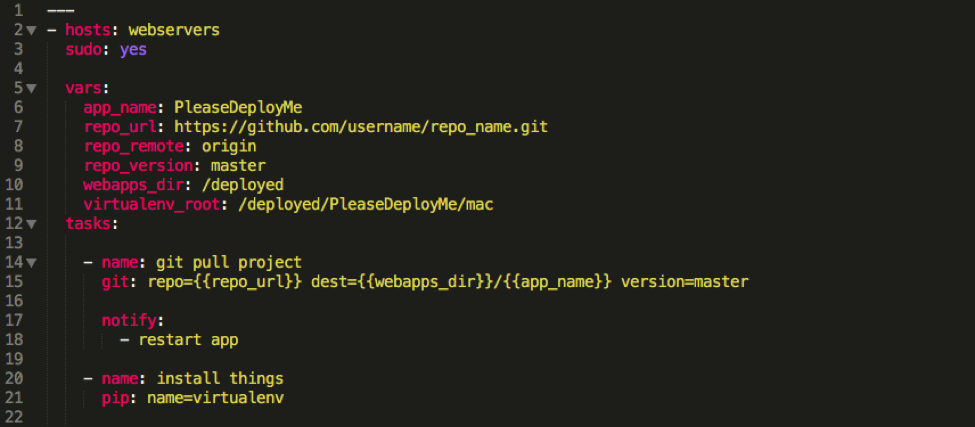
\includegraphics[width=0.9\textwidth]{images/playbookex.png}}
    \caption{Voorbeeld van een Ansible playbook.}
    \label{fig:playbook}
\end{figure}

Ansible is geschreven zodat als ze de playbook uitvoeren ook checken of deze task nog moet gedaan worden. Bijvoorbeeld als een Ansible taak is om een webserver op te starten, zal Ansible deze alleen uitvoeren als de webserver nog niet is opgestart. Dit staat bekend als idempotente. Het zorgt ervoor dat de configuratie altijd snel en efficiënt wordt uitgevoerd.

Met Ansible kan je taken ook inkapselen in een role. Dit wordt gebruikt als je een specifieke configuratie meerdere keren moet uitvoeren, bijvoorbeeld het opzetten van een webserver. De Ansible Galaxy site bevat veel roles die kunnen gebruikt en aangepast worden voor het gebruik in een playbook.
\begin{figure}[!htb]
    \center{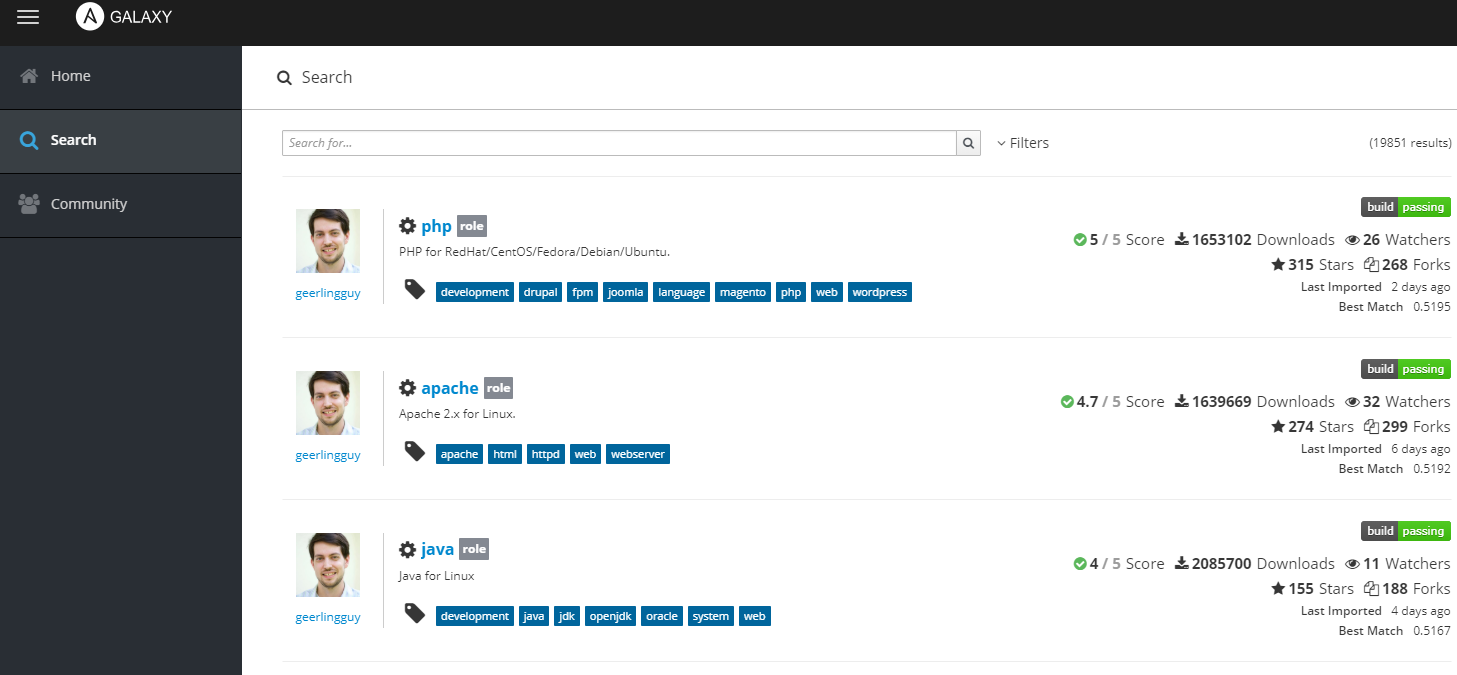
\includegraphics[width=0.9\textwidth]{images/agalaxy.png}}
    \caption{Ansible Galaxy site met lijst van roles.}
    \label{fig:agalaxy}
\end{figure}


\subsection{Omgevingen}
Ansible is zeer makkelijk te deployen cloud omgevingen als publieke of private cloud omgeving op cloud providers als Amazon Web Services, Microsoft Azure, Rackspace,... Maar ook op lokale infrastructuren zoals Virtualbox, VMware,... Hier behoren niet alleen  compute provision, maar ook opslag en netwerken.


